\deu{\section{Datenanalyse}\index{Datenanalyse}}
\eng{\section{Data analysis}\index{Data analysis}}
\setcounter{aufgabenNummer}{300}
\renewcommand{\kAufgabenBuchstabe}{D}

\isAufgaben{
\subsection{\deu{Vorbemerkungen}\eng{Preliminaries}}
\deu{\paragraph{Abkürzungen}}\eng{\paragraph{Abbrevations}}

$n$ = \deu{Anzahl Werte = Stichprobenumfang}\eng{Sample size}

$Q_1$ = \deu{erstes Quartil}\eng{first quartile} 


$IQR$ = Interquartile range (IQR) \deu{= Quartilsdifferenz (QD)} = $Q_3 - Q_1$

$\varsigma$ = \deu{Standardabweichung}\eng{Standard Deviation}

$\overline{x}$ = \deu{empirischer Mittelwert}\eng{average}

$med$ = Median

$Q_3$ = \deu{drittes Quartil}\eng{third quartile} 

$R$ = Range\deu{ = Spannweite}
}


\kKommentar{Sättigung etc. einmal mit e einmal ohne und umgekehrt.}

\subsection{\deu{Grundlagen}\eng{Basics}}

%% %%%%%%%%%%%%%%%%%%%%%%% Aufgabe %%%%%%%%%%%%%%%%%%%%%%%%%%%%%%%%%%%%%%%%%%%%%%%%

\kNiveauAufgabe{

\deu{Das Säulendiagramm zeigt die Anzahl Kinder pro Familie in einer Siedlung mit
$n=150$ Familien (10 Familien haben keine Kinder, 25 Familien haben 1
  Kind, ...).

\makebox{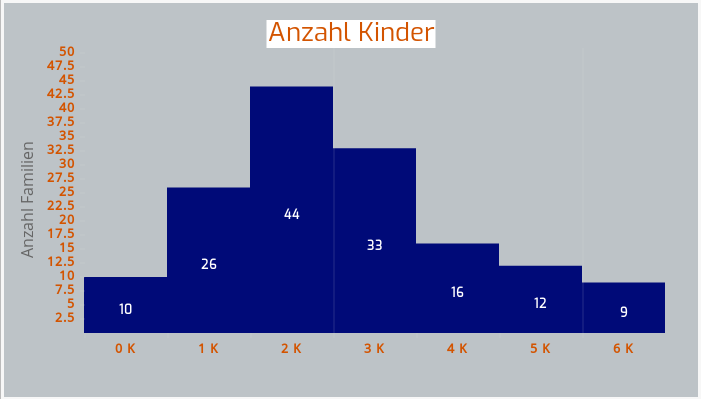
\includegraphics[width=10cm]{img/stoch/statistic_anz_familien_anz_kinder.png}}

a) Berechnen Sie die relativen Häufigkeiten als Dezimalzahl (3
Dezimalen) und in Prozenten (1 Dezimale).

b) Berechnen Sie die durchschnittliche Kinderzahl pro Familie

c) Erklären Sie anhand dieses Beispiels die Begriffe

\begin{itemize}
\item
\textit{Stichprobenumfang\index{Stichprobe}\index{Stichprobenumfang}
\item
Merkmalsträger\index{Merkmalsträger},
\item
Merkmal\index{Merkmal}
\item
Merkmalsprägung\index{Merkmalsprägung}
\item 
  absolute Häufigkeit\index{absolute
    Häufigkeit}\index{Häufigkeit!absolute}
    \item
    relative
  Häufigkeit\index{relative Häufigkeit}\index{Häufigkeit!relative}}
\end{itemize}

d) Wie viele Kinder leben in dieser Siedlung?}%% end deu

\eng{The bar chart shows the number of children per family in a settlement with $n=150$ families (10 families have no children, 25 families have 1 child, ...).

\makebox{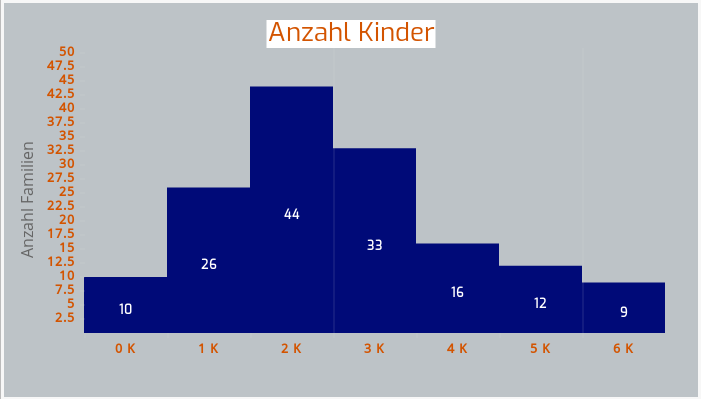
\includegraphics[width=10cm]{img/stoch/statistic_anz_familien_anz_kinder.png}}

a) Calculate the relative frequencies as decimal numbers (3 decimals) and in percentages (1 decimal).

b) Calculate the average number of children per family.

c) Explain the terms using this example:

\begin{itemize}
\item
Sample size
\item
Feature carrier
\item
Feature manifestation
\item
Absolute frequency
\item
Relative frequency
\end{itemize}

d) How many children live in this settlement?}%% end eng
\kVerweiseAltesKompendium{36}{1}
\kPlatzFuerBerechnungen{10}
}{% Lösungen
a)

\begin{tabular}{|c|c|c|c|c|c|c|c|}\hline
\deu{Anzahl Kinder}\eng{number of childs}       & 0      & 1     & 2     &  3    & 4     & 5      & 6   \\\hline
\deu{Relative Häufigkeit}\eng{relative frequency} & 0.063  & 0.173 & 0.293 & 0.220 & 0.107 & 0.080  & 0.060     \\\hline
in \%               & 6.3    & 17.3  & 29.3  & 22.0  & 10.7  & 8.0    & 6.0 \\\hline
 \end{tabular} 

b) $\overline{x} \approx 2.61 $ \deu{Kinder pro Familie}\eng{childs
per family}

c) \deu{Siehe Theorie}\eng{see theory}

d) \deu{Es leben 391 Kinder in der Siedlung.}
\eng{391 children live in the settlement.}

}


%% %%%%%%%%%%%%%%%%%%%%%%% Aufgabe %%%%%%%%%%%%%%%%%%%%%%%%%%%%%%%%%%%%%%%%%%%%%%%%

\kNiveauAufgabe{
\deu{Gegeben sind folgende Rohdaten:}
\eng{The given raw data is as follows:}
  7, 5, 3, 8, 1, 2, 10, 5, 8, 9, 2


  \begin{enumerate}[label=\alph*)]
  \item \deu{Erstellen Sie eine geordnete Liste.}\eng{Create an ordered list.}
  \item \deu{Auf welchem Rang\index{Rang} befindet sich der Wert 3?}\eng{On which rank\index{rank} does the value 3 appear?}
    \item \deu{Welcher Wert befindet sich auf dem mittleren Rang?}\eng{What value is at the median rank?}
  \end{enumerate}


\kVerweiseAltesKompendium{36}{2}
  \kPlatzFuerBerechnungen{8}
}{%% Lösungen
a) 1 , 2 , 2 , 3 , 5 , 5 , 7 , 8 , 8 , 9 , 10

b) \deu{Auf dem 4. Rang.}\eng{On rank 4.}

c) Median: $\mediantilde{x}=5$
}
%%%%%%%%%%%%%%%%%%%%%%%%%%%%%%%%%%%%%%%%%%%%%%%%%%%%%%%%%%%%%%%%%%%%%%%%%%%%%%%%%%%%%%%%%%%%%%%%%%%%%%%%%%%%%%%%%%%%%%555
\subsection{\deu{Datenerhebung: Problematik von Ausreißern}\eng{Data Collection: Issue of Outliers}}

%% %%%%%%%%%%%%%%%%%%%%%%% Aufgabe %%%%%%%%%%%%%%%%%%%%%%%%%%%%%%%%%%%%%%%%%%%%%%%%

\kNiveauAufgabe{
\deu{ Das Durchschnittsvermögen in einer kleinen Gemeinde mit 250
  steuerpflichtigen Personen betrug CHF 175\,600.-.

  Durch den Zuzug einer einzigen vermögenden Person erhöhte sich
  dieser Durchschnitt auf CHF 220\,900.-. Wie hoch ist das Vermögen
  dieser Person?}
  \eng{The average wealth in a small community with 250 taxable
  individuals was CHF 175,600.
  With the arrival of a single wealthy individual, this average
  increased to CHF 220,900.
  What is the wealth of this person?
  }
  \kVerweiseAltesKompendium{37}{3}
  \kPlatzFuerBerechnungen{8}
}{%% Lösung
\deu{Das Vermögen dieser Person ist etwa }
\eng{The wealth of this person is approximately }
         CHF $11\,545\,900.--$.
}


%% %%%%%%%%%%%%%%%%%%%%%%% Aufgabe %%%%%%%%%%%%%%%%%%%%%%%%%%%%%%%%%%%%%%%%%%%%%%%%

\kNiveauAufgabe{
\deu{Das monatliche Durchschnittseinkommen in einer Firma mit 850
  Beschäftigten beträgt CHF 7\,250.-. Die drei Spitzenverdiener dieser
  Firma verdienen monatlich je CHF 86\,000.-.
  Berechnen Sie das monatliche Durchschnittseinkommen, wenn diese drei
  Spitzenwerte nicht berücksichtigt werden.}%% end deu
  \eng{The monthly average income in a company with 850 employees is CHF 7,250. The top three earners in this company each earn CHF 86,000 per month. Calculate the monthly average income if these top three values are not taken into account.}
  \kVerweiseAltesKompendium{37}{4}
  \kPlatzFuerBerechnungen{8}
}{%% Lösung
\deu{Pro nicht-Spiztenverdiener sind das }
\eng{For non-top earners, it is } CHF $6\,971.05$.
}

%% %%%%%%%%%%%%%%%%%%%%%%% Aufgabe %%%%%%%%%%%%%%%%%%%%%%%%%%%%%%%%%%%%%%%%%%%%%%%%

\kTrainingAufgabe{
\deu{
In einer Schulklasse ergaben sich bei der Auswertung einer Prüfung
  folgende Punktezahlen:}%% end deu

\eng{
In a school class, the following scores were obtained in the
evaluation of an exam:}%% end eng


35, 58, 59, 4, 38, 43, 45, 52, 49, 55
\deu{  a) Berechnen Sie Mittelwert und Median.

  b) Berechnen sie den Mittelwert ohne den Ausreißer 4.}%% end deu

\eng{
a) Calculate the mean and median.

b) Calculate the mean without the outlier 4.}%% end eng

  \kVerweiseAltesKompendium{37}{5}
\kPlatzFuerBerechnungen{8}
}{%% Lösung
\deu{Taschenrechner:}\eng{calculator}

 a) \deu{Mittelwert}\eng{average} $\overline{x} =  43.8$ \deu{und
 Median}\eng{and median} $\mediantilde{x} = 47 $

 b) \deu{Mittelwert}\eng{average} $\overline{x} =  48.\overline{2}$

}

%% %%%%%%%%%%%%%%%%%%%%%%% Aufgabe %%%%%%%%%%%%%%%%%%%%%%%%%%%%%%%%%%%%%%%%%%%%%%%%

\kNiveauAufgabe{
\deu{  Zehn Eier haben folgende Gewichte in Gramm:

  52.8, 55.9, 58.2, 57.1, 60.4, 69.1, 57.9, 58.0, 62.5, 65.0

  Nun wird aus Jux zu den Eiern ein Gips-Ei hinzugelegt. Dadurch
  erhöht sich das Durchschnittsgewicht um 3.48 Gramm pro Ei.

  Berechnen Sie das Gewicht des Gips-Eies.

  Runden Sie auf 0.1 Gramm genau.}%% end deu
\eng{Ten eggs have the following weights in grams:

52.8, 55.9, 58.2, 57.1, 60.4, 69.1, 57.9, 58.0, 62.5, 65.0

Now, for fun, a plaster egg is added to the eggs. As a result, the average weight increases by 3.48 grams per egg. Calculate the weight of the plaster egg. Round to 0.1 gram.}%%end eng  
  \kVerweiseAltesKompendium{37}{6}
  \kPlatzFuerBerechnungen{8}
}{%% Lösung
\deu{Das Gips-Ei wiegt 98.0 g (exakt: 97.97g).}%% end deu
\eng{The plaster egg weighs 98.0 g (exactly: 97.97g).}%% end eng
}
\newpage

\deu{\subsection{Diagramme (Säulendiagramm, Histogramm, Boxplot)}}
\eng{\subsection{Charts (Bar Chart, Histogram, Box Plot)}}


%% %%%%%%%%%%%%%%%%%%%%%%% Aufgabe %%%%%%%%%%%%%%%%%%%%%%%%%%%%%%%%%%%%%%%%%%%%%%%%

\kNiveauAufgabe{
\deu{\textbf{Balkendiagramm, Säulendiagramm}}
\eng{\textbf{Bar chart, column chart}}

\kKommentar{Balken hinzugefügt, da nur eine Rotation um $90^\circ$}

\kKommentar{...und im Englischen textuell selten unterschieden}

\deu{
In einer Ausstellung wurden im Laufe einer Woche folgende
  Besucherzahlen ermittelt:}

\eng{In an exhibition, the following visitor numbers were recorded over the course of a week:}

  \begin{tabular}{ccccccc}
    Montag & Dienstag & Mittwoch & Donnerstag & Freitag & Samstag & Sonntag \\
    350    & 321      & 647      & 519        & 844     & 1\,314  & 2\,522
  \end{tabular}


\deu{  Zeichnen Sie ein \textbf{Säulendiagramm} mit den relativen
  Häufigkeiten in \%.}
\eng{Draw a \textbf{bar chart} with the relative frequencies in percentage.
}

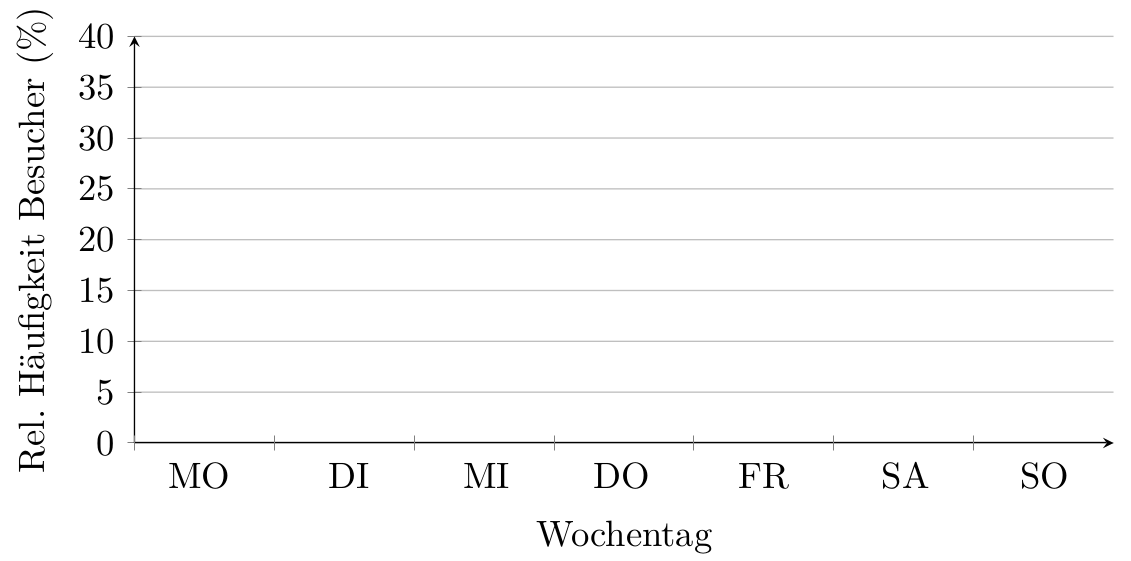
\includegraphics[width=120mm]{img/daan/Museum_Aufgabe.png}

\kVerweiseAltesKompendium{38}{7}
\kPlatzFuerBerechnungen{8}

}{%% Lösung
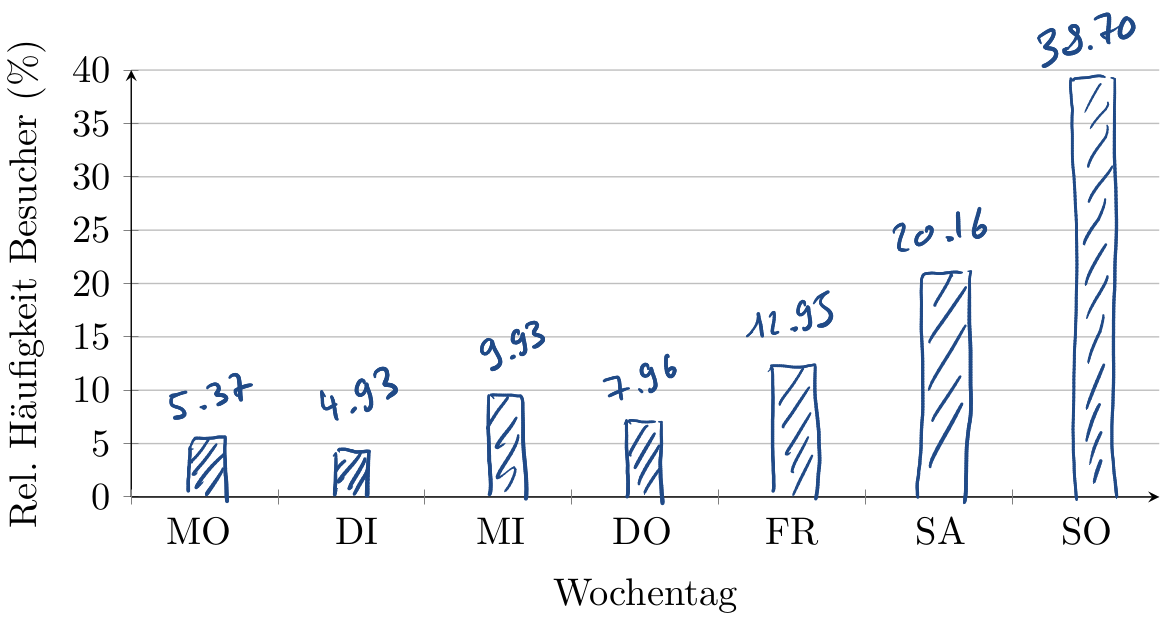
\includegraphics[width=120mm]{img/daan/Museum_Loesung.png}
}
\newpage






%% %%%%%%%%%%%%%%%%%%%%%%% Aufgabe %%%%%%%%%%%%%%%%%%%%%%%%%%%%%%%%%%%%%%%%%%%%%%%%

\kNiveauAufgabe{
 \deu{\textbf{Boxplot und Histogramm}}
 \eng{\textbf{Boxplot and Histogram}}

\kKommentar{Titel Säulendriagramm entfernt}

\kKommentar{Titel Histogramm hinzugefügt}

\deu{Hier sehen Sie die Prüfungspunkte in einer Klasse. Geordnete
Urliste:}
\eng{Here are the exam scores in a class.

Ordered raw data:
}

  52, 62, 66, 72, 74, 74, 76, 76, 76, 78, 80, 82, 82, 84, 86, 88, 92, 96

  \begin{enumerate}[label=\alph*)]
      \item \deu{Bestimmen Sie die \textbf{Quartilsdifferenz} \textit{IQR}.}
            \eng{Determine the \textbf{interquartile range} \textit{IQR}.}
      
      \item \deu{Teilen Sie die Daten in Klassen ein: $[50; 60[$, $[60; 70[$, usw.
        \textit{(Klassenbreite = 10 Punkte).} Zeichnen Sie ein
        Histogramm mit den relativen Häufigkeiten.}%% end deu
        \eng{Divide the data into classes: $[50; 60[$, $[60; 70[$, etc.
\textit{(Class width = 10 points).} Draw a histogram with the relative frequencies.}
      \item
        \deu{Zeichnen Sie einen \textbf{Boxplot}.} \eng{Draw a \textbf{box plot}.} 
      \item
        \deu{Bestimmen Sie den \textbf{Mittelwert}.}\eng{Determine the \textbf{mean}.}
      \item
       \deu{Bestimmen sie den \textbf{Modalwert} (Modus).}\eng{Determine the \textbf{mode} (modal value).}
    \end{enumerate}
%%    \mmPapierZwei{6}{17.5}
\begin{tabular}{c}
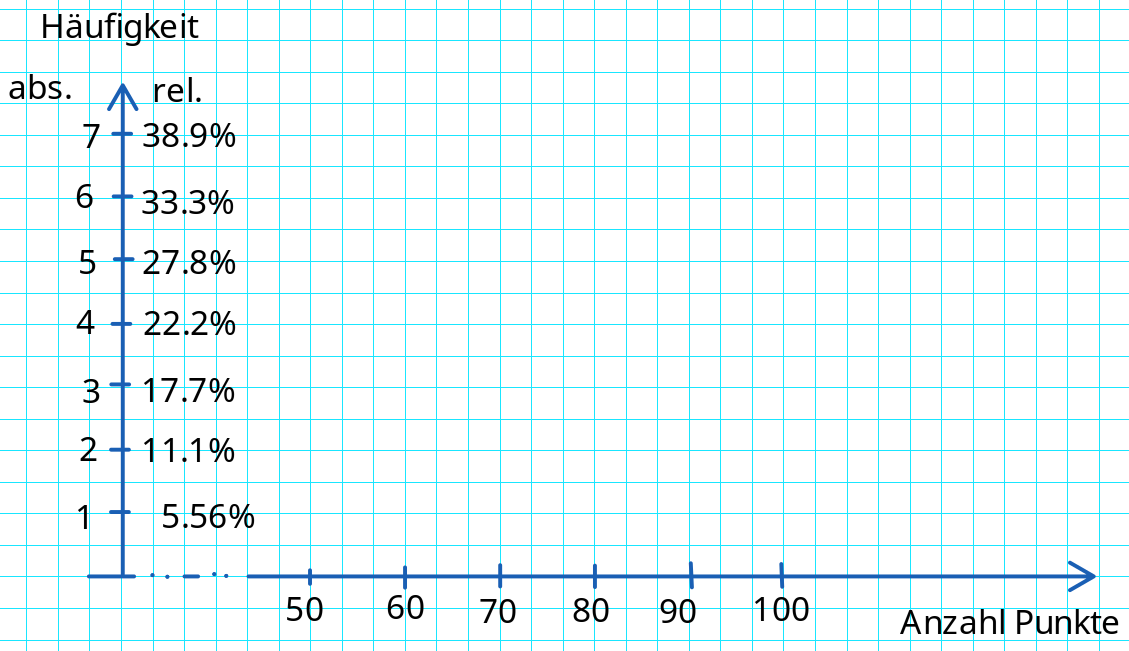
\includegraphics[width=100mm]{img/daan/HistogrammLeer.png} \\
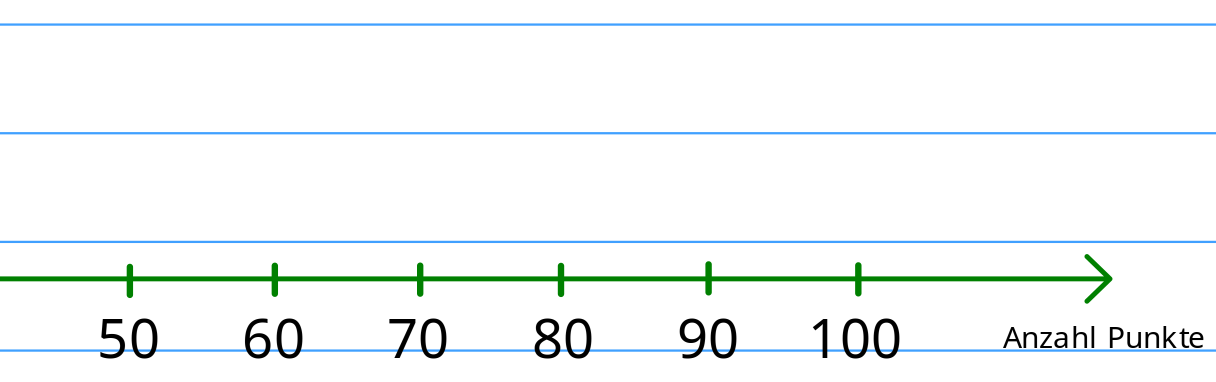
\includegraphics[width=120mm]{img/daan/BoxplotLeer.png}
 \end{tabular}
\newpage 
\kVerweiseAltesKompendium{38}{8}
\kPlatzFuerBerechnungen{8}

}{%% Lösung
a) Median = 76.5; Q1 = 74;  Q3 = 84 und IQR(=QD)=10

   \deu{Maximale Whisker-Länge ist somit 15 und die obere Ausreisserschwelle
   liegt bei 99 und die untere Ausreisserschwelle bei 59. Somit ist
   nur unten ein Ausreißer zu finden.}
   \eng{The maximum whisker length is 15, and the upper outlier
   threshold is 99, while the lower outlier threshold is
   59. Therefore, there is only an outlier on the lower side.}
   
b) c)

\begin{tabular}{cc}
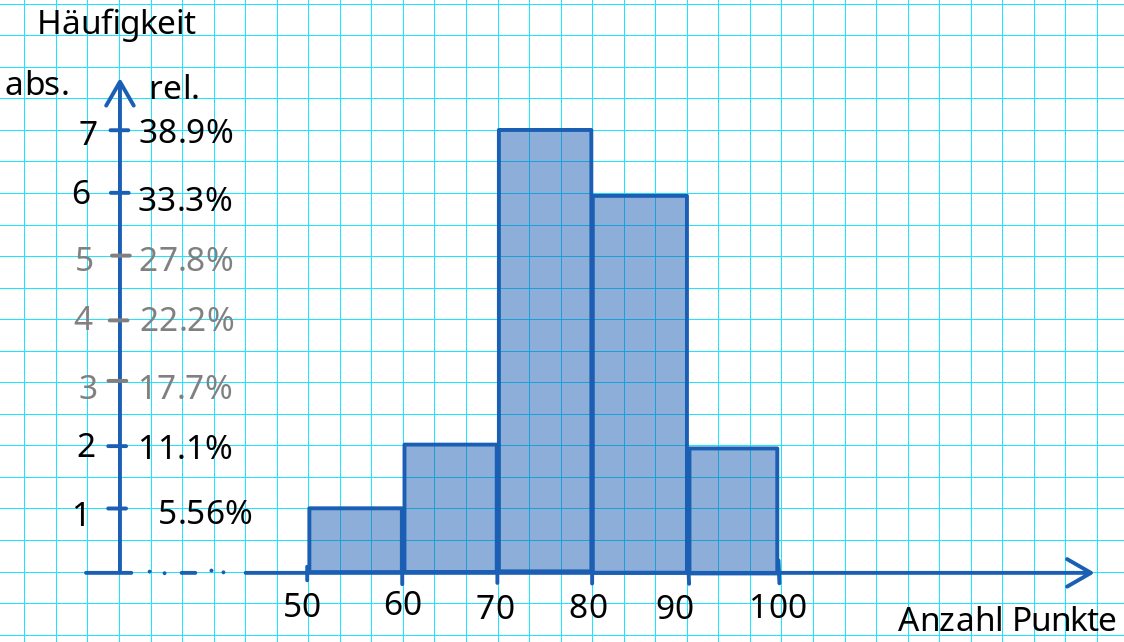
\includegraphics[width=88mm]{img/daan/HistogrammVoll.png} & 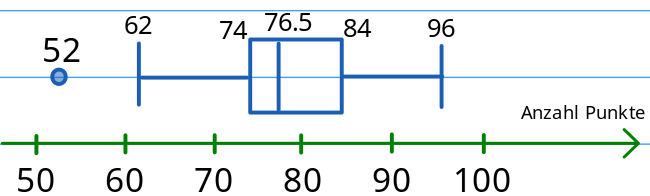
\includegraphics[width=74mm]{img/daan/BoxplotVoll.png}
 \end{tabular}

d) \deu{Summe}\eng{Sum} = 1396. \deu{Mittelwert}\eng{mean} = 77.555.. \deu{Punkte}\eng{points}

e) \deu{Der Modus ist 76, die Zahl kommt drei mal vor.}\eng{The mode is 76, and the number occurs three times.}
}






%% %%%%%%%%%%%%%%%%%%%%%%% Aufgabe %%%%%%%%%%%%%%%%%%%%%%%%%%%%%%%%%%%%%%%%%%%%%%%%




\kNiveauAufgabe{
\deu{\textbf{Klasseneinteilung, Histogramm, Boxplot}}
\eng{\textbf{Class Division, Histogram, Box plot}}


\kKommentar{Klassendiagramm wird Klasseneinteilung}

\kKommentar{Säulendiagramm in Histogramm geändert}

 \deu{Die Messung der Körpergrösse von 100 18-jährigen Schülern liefert
 folgende Zahlen:}
\eng{The measurement of the height of 100 18-year-old students
 provides the following numbers:}
 
\vspace{5mm}

\begin{tabular}{lc|c|c|c|c|c|c|c|c|c}
   \deu{Grösse}\eng{Height} in cm & 163 & 164 & 165 & 166 & 167 & 168 & 169 & 170 & 171 & 172\\\hline
   \deu{Anzahl}\eng{Count}      &  1  &  1  &  1  &  3  &  3  &  3  &  4  &  6  &  5  &  5
   \end{tabular}

\vspace{5mm}


 \begin{tabular}{lc|c|c|c|c|c|c|c|c|c}
   \deu{Grösse}\eng{Height} in cm & 173 & 174 & 175 & 176 & 177 & 178 & 179 & 180 & 181 & 182\\\hline
   \deu{Anzahl}\eng{Count}      &  4  &  7  &  6  &  5  &  5  &  7  &  5  &  4  &  4  &  6
   \end{tabular}

\vspace{5mm}

  \begin{tabular}{lc|c|c|c|c|c}
   \deu{Grösse}\eng{Height} in cm & 183 & 184 & 185 & 186 & 187 & 188\\\hline
   \deu{Anzahl}\eng{Count}      &  5  &  3  &  3  &  2  &  1  &  1 
  \end{tabular}

  \begin{enumerate}[label=\alph*)]
  \item \deu{Erstellen Sie eine Klasseneinteilung mit Klassenbreite 5cm:

    Klasse 1: [160cm; 165cm[

    Klasse 2: [165cm; 170cm[

        usw.

        Zeichnen Sie anschliessend ein Histogramm mit den relativen
        Häufigkeiten in Prozent.}%% end deutsch

\eng{Create a class division with a class width of 5cm:

Class 1: [160cm; 165cm[

Class 2: [165cm; 170cm[

etc.

Afterward, draw a histogram with the relative frequencies in percentage.


}%% end englisch

        \item \deu{Zeichnen Sie einen Boxplot mit diesen Daten.}\eng{Draw a box plot with this data.}
        
\end{enumerate}
\kVerweiseAltesKompendium{39}{9}
\kPlatzFuerBerechnungen{8}

}{%% Löusngen

\begin{tabular}{c|c|c|c|c|c|c}
[160;165[ & [165;170[ & [170;175[ & [175;180[ & [180;185[ & [185;190[  & $\Sigma$ \\\hline
    1     &     2     &     8     &    5      &     2     &   18       &     36\\\hline
    2\%   & 14\%      & 27\%      & 28\%      &22 \%      & 7\%       & 100\%\\
 \end{tabular}
 
\begin{tabular}{cc}
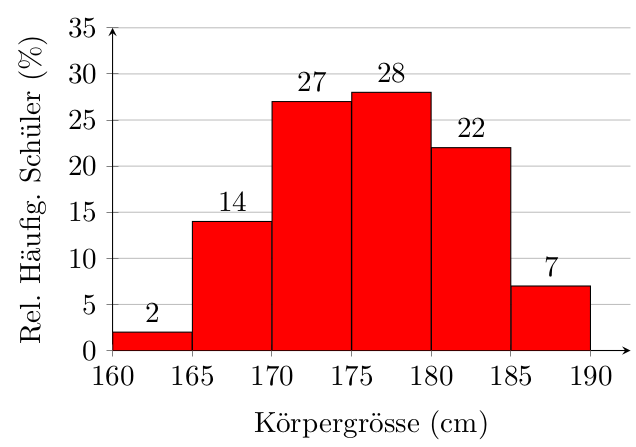
\includegraphics[width=70mm]{img/daan/KoerpergroesseHistogramm.png}
&
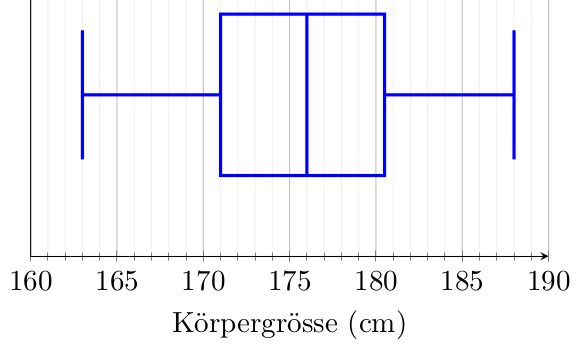
\includegraphics[width=80mm]{img/daan/KoerpergroesseBoxplot.png}
\end{tabular}
}
\newpage









%% %%%%%%%%%%%%%%%%%%%%%%% Aufgabe %%%%%%%%%%%%%%%%%%%%%%%%%%%%%%%%%%%%%%%%%%%%%%%%



\kNiveauAufgabe{
\deu{\textbf{Vergleich zweier Boxplots}}
\eng{\textbf{Comparison of Two Boxplots}}

\deu{Wurfweiten beim Ballwurf in Metern:}\eng{Throw distances (balls) in meters:}

\deu{Versuchsreihe 1}\eng{Experimental series 1}:

  34.0, 34.4, 32.2, 33.5, 35.2, 32.9, 32.6, 34.3, 33.2, 34.1,
  33.2, 33.2, 34.0, 32.7. 34.8, 33.5, 33.5

\deu{Versuchsreihe 2}\eng{Experimental series 2}:

  32.8, 33.7, 34,9, 34.3, 34.6, 32.3, 34.0, 33.9, 33.0, 32.4,
  31.1, 35.5, 31.7, 34.8, 33.5, 32.4

 \deu{Erstellen Sie für beide Versuchsreihen je einen Boxplot (Darstellung
  mit gleicher Skala, sodass ein Vergleich möglich wird).}
 \eng{Create a box plot for each experimental series (representation with the same scale to enable comparison).}

\kVerweiseAltesKompendium{40}{10}
\kPlatzFuerBerechnungen{8}

}{%% Lösungen
V1: Q1 = 33.05; Median = 33.5; Q3 = 34.2

V2: Q1 = 32.4; Median = 33.6; Q3 = 34.5

\kKommentar{Aufgaben nochmals lösen:}

Zahlen unbedingt nochmals prüfen, denn die Graphik stimmt nicht (V1
mit V2 tauschen, Q1 und Q3 nochmals kontrollieren, Mittelachse löschen)...

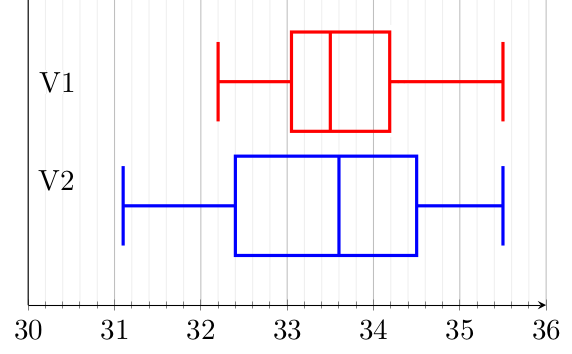
\includegraphics[width=120mm]{img/daan/VergleicheZweiBoxplots.png}

}
\newpage




%% %%%%%%%%%%%%%%%%%%%%%%% Aufgabe %%%%%%%%%%%%%%%%%%%%%%%%%%%%%%%%%%%%%%%%%%%%%%%%

\kKommentar{Mehr Boxplot Aufgaben auch aus alten Prüfungen}

\kKommentar{Auch Boxplotdaten interpretieren}

\newpage

\kNiveauAufgabe{
\deu{
\textbf{Informationen aus einem Diagramm herauslesen}:

Praliné-Kugeln in einer Packung; Darstellung der absoluten
Häufigkeiten in g. Bestimmen Sie die Modalität und die Schiefe des Histogramms.
}%% end deu

\eng{
\textbf{Read information from a diagram}:

Chocolate truffle balls in a package; representation of absolute frequencies in grams. Determine the modality and skewness of the histogram.}%% end eng

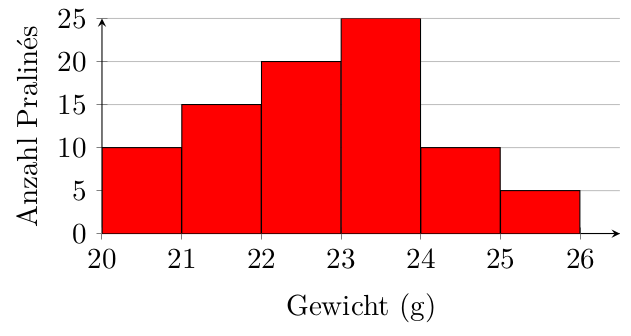
\includegraphics[width=120mm]{img/daan/HistogrammPralines.png}
    
%\begin{tikzpicture}\begin{axis}[ybar stacked,nodes near coords,bar
%    width=0.4,]\addplot
%    coordinates{(21,10) (22,15) (23, 20) (24, 25) (25, 10) (26, 5)};\end{axis}\end{tikzpicture}

%\deu{Bestimmen Sie Mittelwert, Median und Standardabweichung.}
%\eng{Determine mean, median, and standard deviation.}

\kVerweiseAltesKompendium{40}{11}
\kPlatzFuerBerechnungen{8}

}{%% Lösungen
\deu{Unimodal und linksschief (rechtssteil)}
\eng{Unimodal and left-skewed (right-tailed).}
}%% end Aufgabe
\newpage
\kKommentar{Aufgabe mit Säulen}
Beispiel: Alter von Studenten 3x 20j; 4x21j; 6x 22j; 7x23j, 3x24j
2x25j ; 1x26j und 1x 34 j.

Nur Diagramm angeben und Daten wie Median, Mittelwert,
Standardabweichung aus dem Diagramm herauslesen.

\kKommentar{Aufgaben aus den Sozialwissenschaften.}

\newpage

\deu{\subsection{Masszahlen (Mittelwert, Median, Quartile,
  Standardabweichung, Quartilsdifferenz)}}%% end deu

\eng{\subsection{Measurements (Mean, Median, Quartiles, Standard Deviation, Interquartile Range)}}%% end deu

%% %%%%%%%%%%%%%%%%%%%%%%% Aufgabe %%%%%%%%%%%%%%%%%%%%%%%%%%%%%%%%%%%%%%%%%%%%%%%%

\kNiveauAufgabe{

\deu{In einer Klasse wurden folgende 18 Prüfungsnoten erzielt:}
\eng{In a class, the following 18 exam grades were obtained:}

  \begin{tabular}{llllllllll}
    3 & 3 & 3.5 & 3.5 & 4   & 4 & 4.5 & 4.5 & 4.5 & 4.5\\
    5 & 5 & 5.5 & 5.5 & 5.5 & 6 & 6   & 6
  \end{tabular}

  \deu{Berechnen Sie \textbf{Mittelwert} und \textbf{Standardabweichung}
  mit Hilfe des Rechners.}%% end deu
  \eng{Calculate the \textbf{mean} and \textbf{standard deviation} using the calculator.}

\kVerweiseAltesKompendium{41}{12}

\kPlatzFuerBerechnungen{8}

}{%% Lösungen
$\overline{x} = 4.64$, $\sigma=0.97$ (bzw. $s_x=1.0$)
}





%% %%%%%%%%%%%%%%%%%%%%%%% Aufgabe %%%%%%%%%%%%%%%%%%%%%%%%%%%%%%%%%%%%%%%%%%%%%%%%

\kNiveauAufgabe{
\deu{Drei \textbf{Streumasse}: \textbf{Spannweite R (Range)},
  \textbf{Quartilsdifferenz IQR}, \textbf{Standardabweichung
  $\sigma$}}%% end deu

\eng{Three \textbf{dispersion measures}: \textbf{Range R}, \textbf{Interquartile Range IQR}, \textbf{Standard Deviation $\sigma$}}


\deu{Gegeben sind folgende Daten, die bereits geordnet sind:}
\eng{Given are the following data, which are already sorted:}

  \begin{tabular}{llllllllll}
    2.5 & 2.8 & 3.2 & 3.5 & 3.5 & 4.1 & 4.2 & 4.7 & 4.8 & 4.8\\
    5.4 & 5.5 & 6
  \end{tabular}

  \deu{Ermitteln Sie die \textbf{Spannweite (Range)}, die
  \textbf{Quartilsdifferenz QD (Interquartilerange (IQR)) } und die \textbf{Standardabweichung} (auf
  2 Dezimalen genau).}
  \eng{Determine the \textbf{range}, the \textbf{interquartile range (IQR)}, and the \textbf{standard deviation} (to 2 decimal places).
}

\kVerweiseAltesKompendium{41}{13}
\kPlatzFuerBerechnungen{8}
}{%% Lösungen
\eng{Range}\deu{(Spannweite)} = $3.55$, IQR \deu{(Quartilsdifferenz QD)} = $1.75$ und  $\sigma=1.04$ ($s_x=1.09$)
}  

\newpage
